\documentclass[010-intro.tex]{subfiles}

\begin{document}

Many data science students go on to teach,
but are rarely trained in pedagogy \cite{clevelandDataScienceAction2001}.
What is also lacking are rigorous evaluations of data science tools
that statisticians advocate for process improvements in other disciplines
\cite{clevelandDataScienceAction2001}.
Industry and government can use
professional advisory boards, work-study programs, and internships
to generate the demand for modern computational skills
\cite{cc2020}.
Academic institutions can benefit their graduates by proactively
supporting strong, contemporary computing programs \cite{cc2020}.
The discrepancy between student need for clinical informatics courses,
and the availability and opportunity to take a clinical informatics course in the biomedical sciences
\cite{banerjeeMedicalStudentAwareness2015, americanmedicalassociationStudentInterestInformatics},
show that academic institutions, industry, and government
can play a role in meeting training needs for the biomedical sciences.
This dissertation aims to fill the gaps of improving the data process statisticians advocate for,
while also providing a set of learning materials that meet the need for the biomedical sciences.


% Taken from persona chapter intro
Healthcare providers
(e.g., medical doctors, veterinarians, nurses, physician assistants, other clinicians, and administrators)
play a key role in the interdisciplinary needs in health care
\cite{surowiecki2005wisdom, hoytOverviewTwoOpen2018, payneBiomedicalInformaticsMeets2018}.
Being able to work with open collaborative data science platforms,
the healthcare domain experts are able to better understand, utilize, and contribute to the
``wisdom of crowds''
\cite{surowiecki2005wisdom, hoytOverviewTwoOpen2018, payneBiomedicalInformaticsMeets2018}.
A coordinated effort between the biomedical communities and data science communities
is a priority in order to create effective curricular frameworks for mutual understanding
of each respective domain
\cite{payneBiomedicalInformaticsMeets2018}.

% Taken from persona chapter intro
In the United States,
the National Institute of Health (NIH) is responsible for biomedical and public health research.
The NIH has made a strategic data science plan to improve the
storage, management, standardization and publication of biomedical research.
Professional organizations such as the
American Medical Association (AMA),
American Nurses Association (ANA),
American Academy of Physician Associates (AAPA), and
American Veterinary Medical Association (AVMA)
serve as national organizations for medical doctors, nurses, physician associates, and veterinarians.
All of these organizations have made calls for the importance of data science in their respective professions
\cite{payneBiomedicalInformaticsMeets2018, americanmedicalassociationAcceleratingChangeMedical2021, americannursesassociationANAEnterpriseAmerican, owenEthicalIntersectionHealthcare2017, nolenArtificialIntelligenceVeterinary2020, nationalinstitutesofhealthNIHStrategicPlan2020}.
The NIH's strategic data science plan (Figure \ref{fig:nih-ds}) has five (5) main goals and objectives:
(1) data infrastructure,
(2) modernized data ecosystem,
(3) data management, analysis, and tools,
(4) workforce development, and
(5) stewardship and sustainability.

\begin{figure}[htb]
    \centering
    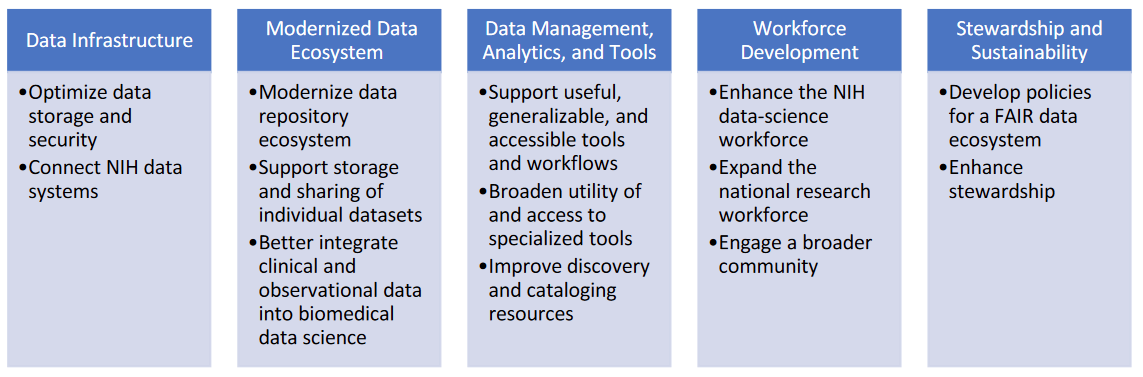
\includegraphics[width=\linewidth]{figs/050-intro/nih-strategic_plan_data_science}
    \caption[NIH Strategic Plan for Data Science]{
    Reproduction of the NIH strategic plan for data science \cite{nationalinstitutesofhealthNIHStrategicPlan2020}.
    The plan consists of five (5) main goals and objectives: (1) data infrastructure,
    (2) modernized data ecosystem,
    (3) data management, analysis, and tools,
    (4) workforce development, and
    (5) stewardship and sustainability.
    The plan's goal is to address the quantity and highly distributed nature of biomedical data and metadata
    that lead to a variety of data formats which lead to data cleaning complications.
    }
    \label{fig:nih-ds}
\end{figure}

The objectives in
data management, analytics, and tools;
workforce development;
and stewardship and sustainability
relate to the more individual data science skills that integrate with larger data infrastructure
\cite{nationalinstitutesofhealthNIHStrategicPlan2020}.

Incorporating computing skills and domain knowledge can be thought of
$\text{computing} + x$ and $x + \text{computing}$ (where $x$ is a knowledge domain)
\cite{cc2020}.
In $\text{computing} + x$, computing systems extend to non-computing disciplines.
These fields usually have ``informatics'' in the term
e.g., medical infomatics, bioinformatics, health informatics, legal informatics, etc \cite{cc2020}.
In $x + \text{computing}$,
computing systems are extensions to an already existing and established field of study.
One prominent example is computational biology,
where established laboratory methods expanded to computing.
Both mechanisms of combining computing and a discipline allow for the discovery of transformational relationships,
only the starting point is different \cite{cc2020}.

Medicine is inherently an information-management task
\cite{shortliffe1993adolescence}.
This dissertation focus on the core and fundamental skills
of data science computing, and how these skills can better areas in the biomedical sciences
($\text{computing} + x$ and $x + \text{computing}$)
by focusing on core data literacy concepts.
By combining domain, computing, and integrative knowledge and skills,
non-computing individuals can make the connections from their domain to the transformative opportunities
created by using computing \cite{cc2020}.

\end{document}
